\chapter{Generative Pattern Database}
% What does this chapter do?
% Sructure
While Section x gives a high-level overview of the proposed architecture, details on the main processing primitives are described in Section x and x. Finally, the algorithms and processes for data transformations and persistence are specified in Section x.

\section{System Architecture}

% Provide a general view on main components and their tasks and interfaces; how is this system supposed to work; how do the components interact with each other
% Specify important definitions on components and data formally


\begin{figure}[t]
    \centering
    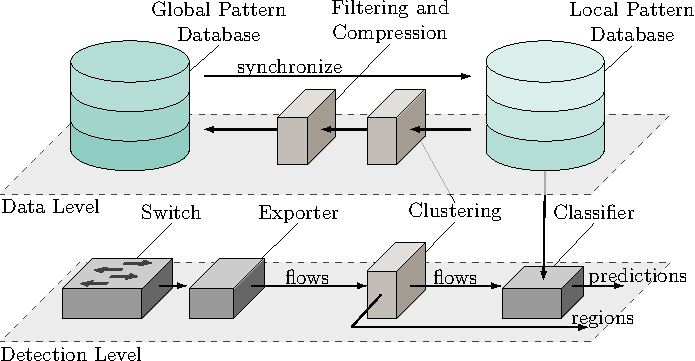
\includegraphics[width=1\linewidth]{tikz/high_level_architecture.pdf}
    \caption{High level CIDS architecture.}
    \label{fig:high_level_architecture}
    \end{figure}

The proposed CIDS exhibits a hierarchical architecture (see Figure \ref{fig:high_level_architecture}). On top, the global infrastructure $G$ provides services, that are globally available to a number of $M \in \mathbb{N}$ local infrastructures $L_m, m \in \{1, \dots, M\}$ that represent the corresponding IT infrastructure boundaries of participating CIDS members. Each $L_m$ agrees to a specified feature extraction process that provides the monitoring data $\bm{X} \subset \mathbb{R}^d$ for attack detection, where specific instances are referred to as $\bm{x} \in \bm{X}$ of size $d = |\bm{x}| \in \mathbb{N}$. In addition, the set of targets $Y \subset \mathbb{N}$ with instances $y \in Y$ is known and registered within each $L_m$. Within every $L_m$, an individual training dataset $D_m= \{(\bm{x}_n, y_n): 1 \leq n \leq N_m\}$ of size $N_m = |D_m| \in \mathbb{N}$ is provided. CIDS communication across local boundaries occurs exclusively in a vertical direction. Thus, the exchange of information between individual $L_m$ takes place indirectly via the global pattern database $(PDB_G)$ and the global event channel $(C_G)$. Each $L_m$ includes a local pattern database $(PDB_{L_m})$, a local event channel $(C_{L_m})$ and an event-based data processing pipeline that consists of four services.



\subsection{Pattern Database} \label{subsec:pattern_database}
Each instance of a pattern database $(PDB)$ is realized as a key-value store. For the following algorithm descriptions, a $PDB$ is treated as a hash table as defined in Section \ref{subsec:hash_table}, referred to by replacing the function variable with the service identifier, e.g. $PDB_G(k)$ being a specific slot or hash value related to a key $k$ in the global pattern database. Note that if a specific hash function is already used to construct a key (e.g. Random Projection), the hash table will internally apply a distinct hash function on the key to ensure even distribution across the slots. 

\subsection{Event Channel} \label{subsec:event_channel}
Event channels provide a topic-based publish-subscribe messaging mechanism that is mainly used to distribute workloads among the service instances in the processing pipeline. Via the messaging system, service instances receive and emit events, on which upon the respective operations are triggered. Changes in a pattern database result in responses that in turn are leveraged as the respective events. In this fashion, updates are propagated throughout the processing pipeline, ensuring a timely consistency among the pattern databases.

\subsection{Processing Pipeline} \label{subsec:processing_pipeline} 
Local and global pattern databases serve exclusively as data sources and sinks for operations. The only exception is the initial import of datasets $D_m$ into the \textit{Local Indexing} service via the messaging system.



\section{Local Indexing}

\begin{figure}[b]
    \centering
    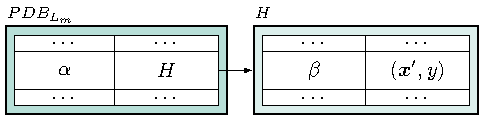
\includegraphics[width=1\linewidth]{tikz/indexing.pdf}
    \caption{Nested indexing in a local pattern database.}
    \label{fig:indexing}
\end{figure}

The local indexing service listens on $C_{L_m}$ for new data points from $D_m$. First, data points are buffered until a defined batch size is released. Subsequently, the batch $X$ is scaled to the range $[-1, 1]$ by applying a feature-wise min-max normalization, given by

\begin{align*}
    \bm{X}' = \frac{\bm{X}-min(\bm{X})}{max(\bm{X}) - min(\bm{X})} \cdot (b - a) + a, \quad
    \setlength\arraycolsep{2pt}
    \begin{array}{lr}
        a = &-1 \\
        b = & 1    
    \end{array}.
\end{align*}

After that, each element $\bm{x}' \in \bm{X}'$ is subject to both a \textit{GRP} $h$ with a global seed for the initialization of the projection plane $\bm{M}$ (see Section \ref{subsec:gaussian_random_projection}) and a non-cryptographic hashing function $g$ (see Section \ref{subsubsec:non-cryptographic-hashes}). The \textit{GRP} clusters the data by mapping similar data points $\bm{x}'$ to the same hash value. The non-cryptographic hashing function on the other hand serves as a mechanism for deduplicating identical $\bm{x}'$. In order to insert a pair $(\bm{x}'_n, y_n) \in D_m$ into the $PDB_{L_m}$, at first two keys $k_\alpha, k_\beta \in K$ are constructed as

\begin{align*}
    k_\alpha(\bm{x}'_n, y_n) &= p_x \doubleplus h(\bm{x}'_n) \doubleplus y_n,\\
    k_\beta(\bm{x}'_n) &= g(\bm{x}'_n),
\end{align*}

where $\doubleplus$ indicates the concatenation operator and $p_x$ describes an arbitrary prefix constant. Secondly, if not already present, a hash table $T_{m_n}$ is created and inserted into the slot $PDB_{L_m}(k_\alpha(\bm{x}'_n, y_n))$. Finally, $(\bm{x}'_n, y_n)$ is hashed into the slot $T_{m_n}(k_\beta(\bm{x}'_n))$. That nested indexing is depicted in Figure \ref{fig:indexing}. Since a particular $h(\bm{x}')$ is a cluster of similar data points, we refer to it as a \textit{region}. Therefore, every region is represented by one or more hash tables $T_{m_n}$, each of them containing data points that belong to the same label. Each execution of that insert operation is executed idempotently, such that the pattern database only returns a response upon the insertion of new data points. For each response, the corresponding region $h(\bm{x}'_n)$ is sent into the local event channel $C_{L_m}$ as an event that indicates a change on a certain cluster within the local pattern database.

\section{Complexity Estimation}

A region is said to be complex, if it contains more than one unique label. Otherwise, a region is simple. Since the data within a region already represents a cluster, the existence of multiple classes indicates a more complex decision boundary. On that basis we differentiate how a region is processed in the subsequent services of the pipeline. Furthermore, the complexity state of a region may vary, depending on the scope it is observed. Note that since the projection matrix $\bm{M}$ is initialized with the same values in every $L_m$, all hashes that were computed by $h$ are globally comparable. This means that similar data points from different datasets, e.g. $\bm{x}_i \in D_1$ and $\bm{x}_j^* \in D_2$ may be hashed to the same region $h(\bm{x}_i) = h(\bm{x}^*_j)$. However, it is also possible that that the corresponding labels $y_i \in D_1$ and $y^*_j \in D_2$ are not equal and therefore lead to a different global view on that region's complexity state. Given that, the complexity estimation module acts as a bridge between the local and global components and answers the question, which regions are considered to be complex in a global context. First, an event containing a region $h(\bm{x}'_n)$ is received. This event is then used for retrieving the set of unique labels $Y_{h(\bm{x}'_n)}$ for that particular region stored at $PDB_{L_m}$, which is defined as

 \begin{align*}
    \bigcup_{y \in Y} \! \Bigl\{ y_n \! \in \! \bigl\{T_{m_n}\bigl(k_\beta(\bm{x}'_n)\bigl)\bigl\} : \! T_{m_n} \! \! \in \! \bigl\{PDB_{L_m}\bigl(k_\alpha(\bm{x}'_n, y) \bigl)\bigl\}\Bigl\}.
 \end{align*}

 Next, a key $k_\gamma \in K$ is constructed by concatenating an arbitrary prefix constant $p_y$ with the region $h(\bm{x}'_n)$ and the id of the current local infrastructure $m$:

\begin{align*}
    k_\gamma(h(\bm{x}'_n), m) = p_y \doubleplus h(\bm{x}'_n) \doubleplus m.
\end{align*}

 Then, $Y_{h(\bm{x}'_n)}$ is inserted into the global pattern database at the slot $PDB_G(k_\gamma(h(\bm{x}'_n), m))$. The global complexity $c_{h(\bm{x}'_n)} \in \{0, 1\}$ is determined by combining the respective label sets from all local infrastructures and evaluating its cardinality:
 
 \begin{align*}
    c_{h(\bm{x}'_n)} = \Bigl| \bigcup_{m \in M} \Bigl\{ PDB_G\bigl(k_\gamma(h(\bm{x}'_n), m)\bigl) \Bigl\}\Bigl| > 1.
 \end{align*}

 Finally, the state $c_{h(\bm{x}'_n)}$ is inserted in the global pattern database by constructing a key $k_\kappa \in K$ with a prefix constant $p_c$ and the region $h(\bm{x}'_n)$ as

 \begin{align*}
     k_\kappa(h(\bm{x}'_n)) = p_c \doubleplus h(\bm{x}'_n)
 \end{align*}

and storing it in the slot $PDB_G(k_\kappa(h(\bm{x}'_n)))$. If the state has changed, a response is returned and the corresponding region $h(\bm{x}'_n)$ is sent as an event into the global event channel $C_G$.

\section{Generative Fitting}

\section{Classifier Fitting}